% This example is meant to be compiled with lualatex or xelatex
% The theme itself also supports pdflatex
\PassOptionsToPackage{unicode}{hyperref}
\documentclass[aspectratio=1610, 9pt]{beamer}

% Load packages you need here
\usepackage{polyglossia}
\setmainlanguage{german}

\usepackage{csquotes}


\usepackage{amsmath}
\usepackage{amssymb}
\usepackage{mathtools}

\usepackage{hyperref}
\usepackage{bookmark}

\usepackage{xfrac}
\usepackage[shortcuts]{extdash}

\usepackage[
  backend=biber,
]{biblatex}
% Quellendatenbank
\addbibresource{lit.bib}

\usepackage[
  locale=DE,                   % deutsche Einstellungen
  separate-uncertainty=true,   % immer Fehler mit \pm
  per-mode=symbol-or-fraction, % / in inline math, fraction in display math
]{siunitx}

\usepackage{svrsymbols}
\usepackage{cancel}

% \AtBeginSection[]{
  % \frame{
    % \frametitle{Inhaltsverzeichnis}
      % \tableofcontents[currentsection]
  % }
% }

% load the theme after all packages

\usetheme[
  showtotalframes, % show total number of frames in the footline
]{tudo}

% Put settings here, like
\unimathsetup{
  math-style=ISO,
  bold-style=ISO,
  nabla=upright,
  partial=upright,
  mathrm=sym,
}

\title{W-Massenmessung}
\author[Julia ~Sobolewski]{Julia Sobolewski}
\institute[Fakultät Physik]{Fakultät Physik}
\titlegraphic{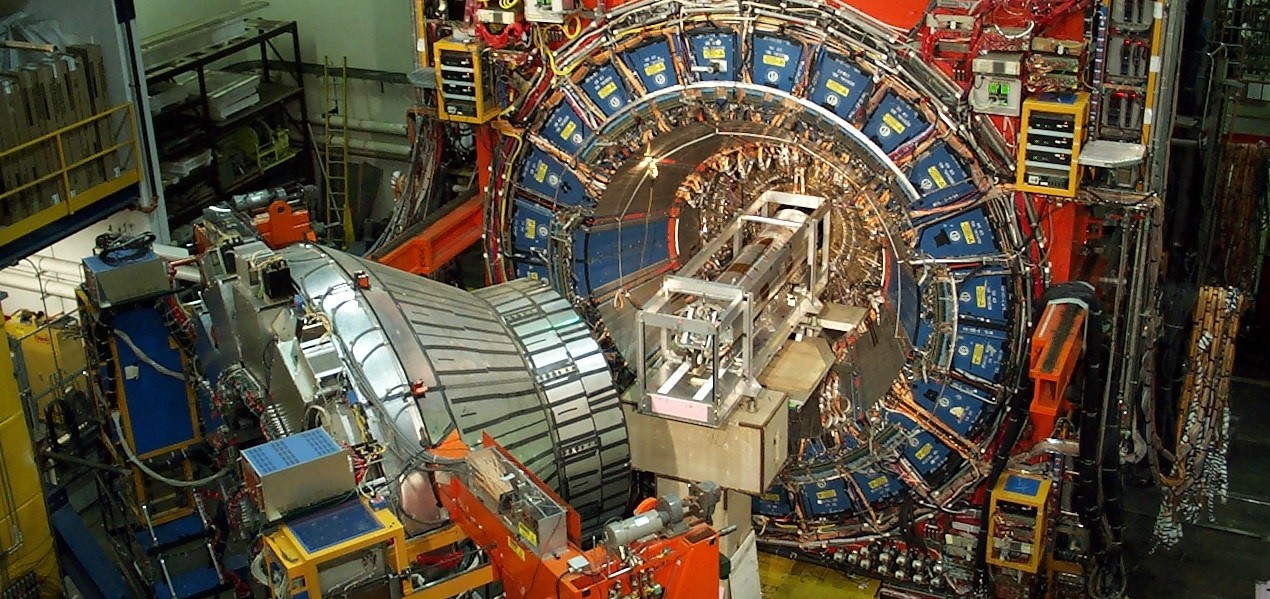
\includegraphics[width=0.7\textwidth]{images/cdf.jpg}}


\begin{document}

\maketitle

\begin{frame}[allowframebreaks]{Inhaltsverzeichnis}
  \tableofcontents
\end{frame}

\section{Einleitung}

\subsection{Was sind W-Bosonen?}

\begin{frame}{Was sind W-Bosonen?}
  \begin{columns}
    \begin{column}{0.4\textwidth}
      \begin{figure}
        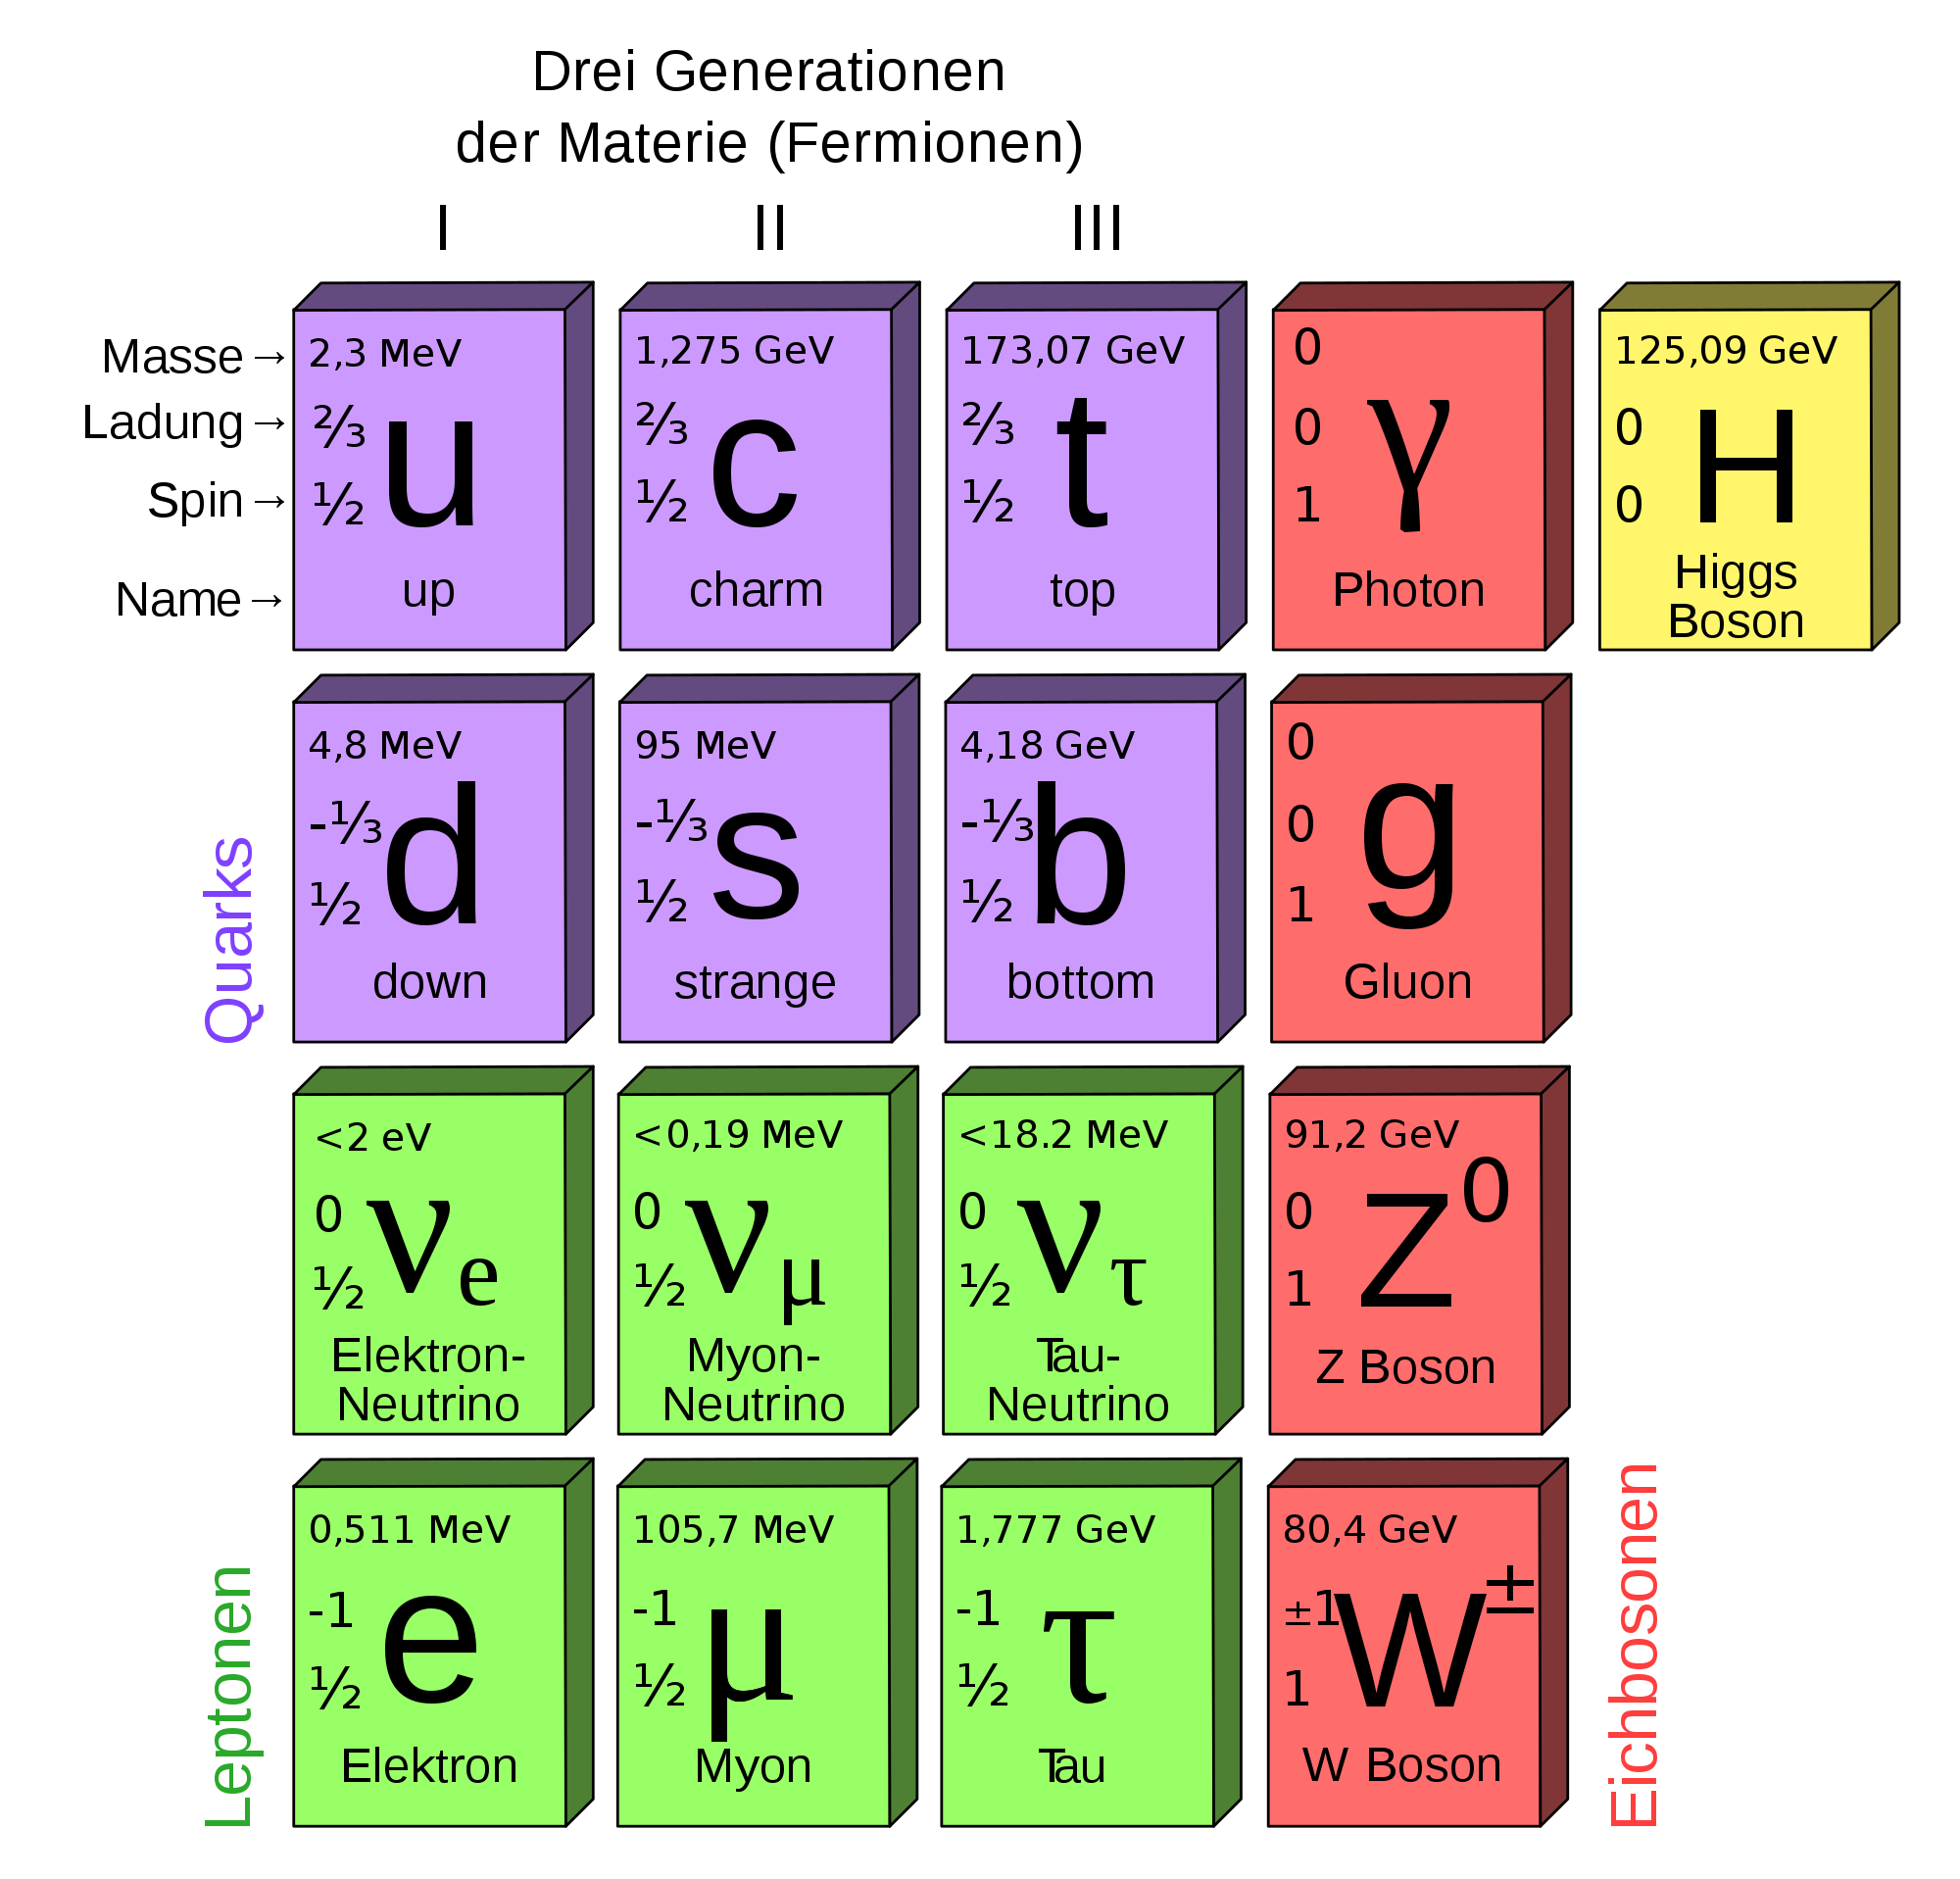
\includegraphics[width=\textwidth]{images/standard_model.png}
        \caption{Standardmodell der Teilchenphysik \cite{standard_model}}
        % \label{}
      \end{figure}
    \end{column}
    \begin{column}{0.4\textwidth}
      \begin{itemize}
        \item Eichboson \rightarrow Elementarteilchen
        \item vermittelt in der elektroschwachen Theorie die geladenen Ströme
        \item Ladung: $q = \pm e$
        \item Spin: $s = 1$
        \item mittlere Lebensdauer: $\SI{3e-25}{\s}$
        \item Masse: $m_W = \SI{80.379(12)}{\GeV}$
      \end{itemize}
    \end{column}
  \end{columns}
\end{frame}

\subsection{Entdeckung des W-Bosons}
\begin{frame}{Entdeckung des W-Bosons}
  \begin{columns}
    \begin{column}{0.4\textwidth}
      \begin{figure}
        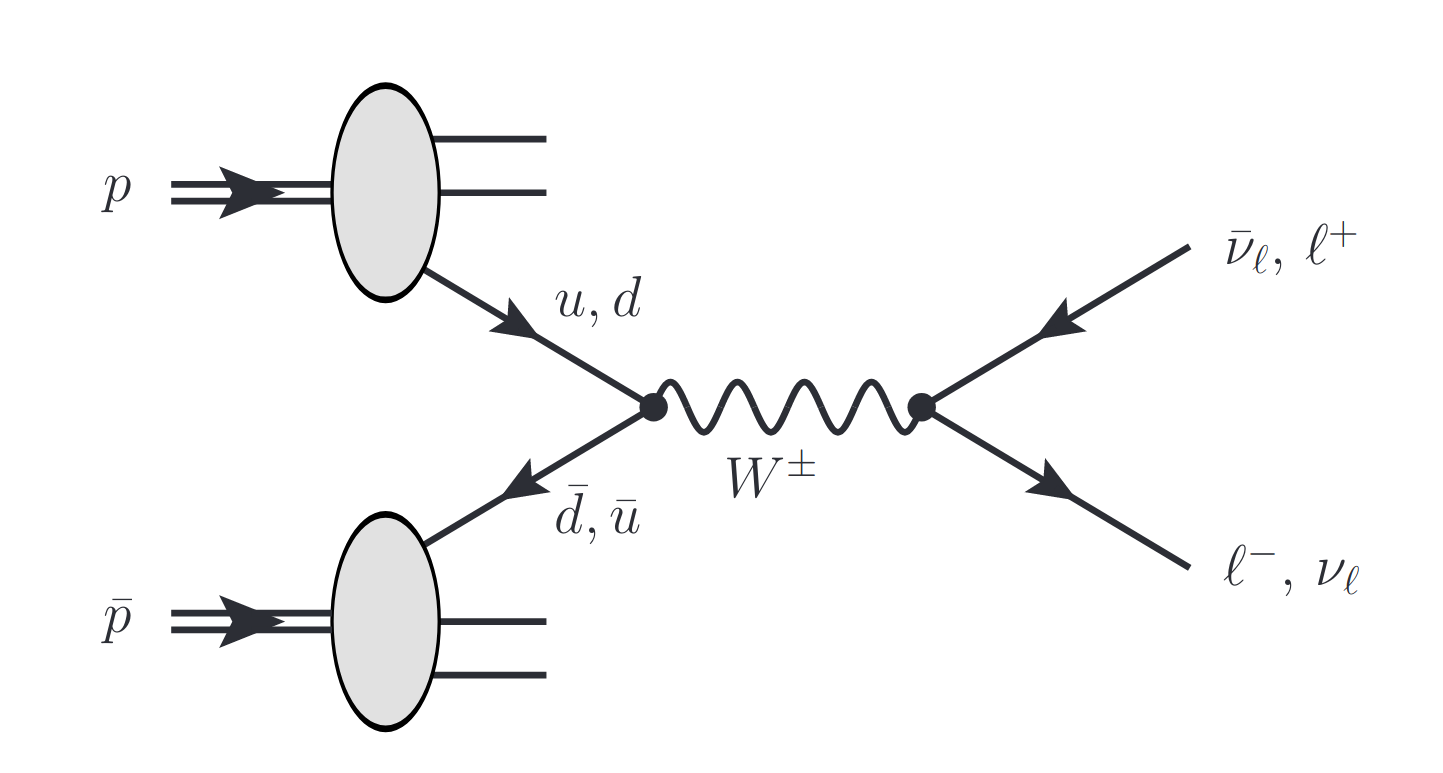
\includegraphics[width=\textwidth]{images/feynman.png}
        \caption{Feynman-Diagramm niedrigster Ordnung zur Erzeugung von W-Bosonen \cite{skript}}
        \label{fig:feynman}
      \end{figure}
    \end{column}
    \begin{column}{0.4\textwidth}
      \begin{itemize}
        \item 1983 am Super Proton Synchrotron (SPS)
        \item Im naiven Partonmodell entsteht das W-Boson bei Kollision eines Valenzquarks des Protons $(\quarku, \quarkd)$ mit einem Valenzantiquark des Antiprotons $(\antiquarku, \antiquarkd)$
        % \item Valenzquark und -antiquark tragen je einen Impulsanteil von $x_{1,2} \approx \SI{0,2}{}$ des (Anti-)Protons
        % \item Benötigte Parton-Parton-Schwerpunktsenergie $\sqrt{\hat{s}} = \SI{80}{\GeV}$ \rightarrow benötigte $\proton \antiproton$-Schwerpunktsenergie $\sqrt{s} = \sqrt{\frac{\hat{s}}{x_1 x_2}} \approx \SI{400}{\GeV}$
      \end{itemize}
    \end{column}
  \end{columns}
\end{frame}

\begin{frame}
  \begin{itemize}
    \item Valenzquark und -antiquark tragen je einen Impulsanteil von $x_{1,2} \approx \SI{0,2}{}$ des (Anti-)Protons
    \item Um ein W-Boson zu erzeugen, wird eine Parton-Parton-Schwerpunktsenergie von $\sqrt{\hat{s}} = \SI{80}{\GeV}$ und somit eine $p \bar{p}$-Schwerpunktsenergie von $\sqrt{s} = \sqrt{\frac{\hat{s}}{x_1 x_2}} \approx \SI{400}{\GeV}$ benötigt
    \item Solche Schwerpunktsenergien waren zuerst am SPS vorhanden ($\sqrt{s} = \SI{540}{\GeV}$)
  \end{itemize}
\end{frame}

\subsection{Motivation}
\begin{frame}{Motivation}
  \begin{columns}
    \begin{column}{0.5\textwidth}
      \begin{figure}
        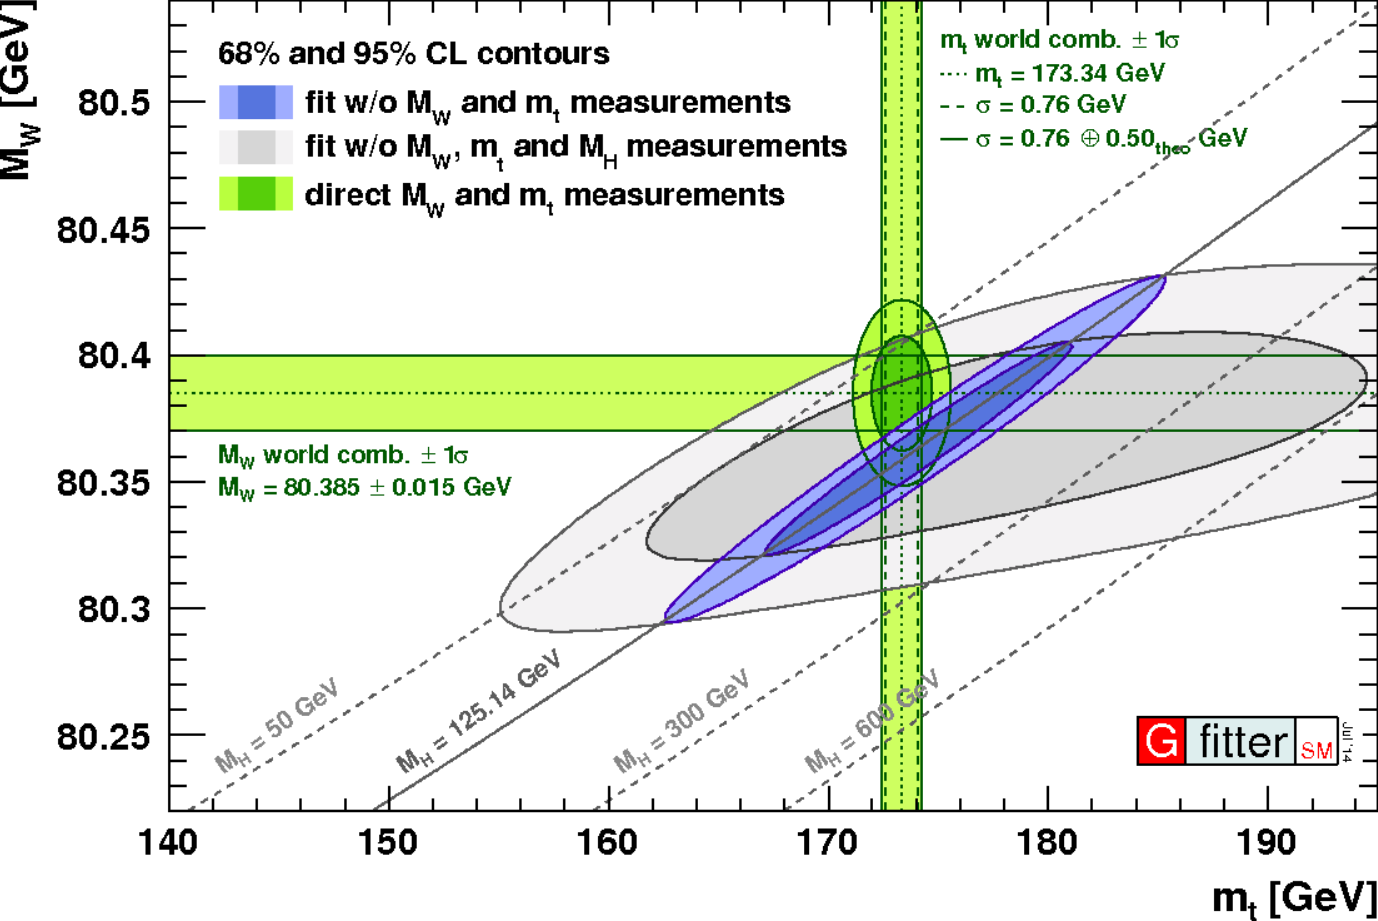
\includegraphics[width=\textwidth]{images/gfitter.png}
        \caption{Fit der schwachen Wechselwirkung \cite{gfitter}}
        \label{fig:gfitter}
      \end{figure}
    \end{column}
    \begin{column}{0.4\textwidth}
      \begin{itemize}
        \item W- und Z-Masse bestimmen zusammen den schwachen Mischungswinkel
        \item durch genaue Kenntnis der W- und t-Masse lässt sich die Masse des Higgs-Bosons eingrenzen
      \end{itemize}
    \end{column}
  \end{columns}
\end{frame}

\subsection{Theoretische Grundlagen}
\begin{frame}{Theoretische Grundlagen}
   \begin{itemize}
     \item Im Gegensatz zum Z-Nachweis im Zerfall $Z \rightarrow \ell^+ \ell^-$ über die invariante Masse des Leptonpaares kann man hier die Vierervektoren der Zerfallsprodukte nicht vollstandig bestimmen
     \item longitudinaler Impuls $p_z$ des Schwerpunktsystems der Kollision ist, weil das System geboostet ist, nicht bekannt \\
     \item[$\longrightarrow$] Lösung: Verwendung transversaler Größen
   \end{itemize}
\end{frame}

\begin{frame}
  \begin{itemize}
    \item im Zerfall $W \rightarrow \ell \nu$ insbesondere die Transversalimpulse des Leptons $p^\ell_T$ und des Neutrinos $p^\nu_T$ von besonderem Interesse
    \item Der Transversalimpuls des Neutrinos kann nur indirekt über "fehlende transversale Energie"  $\cancel{\it{E}}_{T}$ bestimmt werden
    \item Wenn man annimmt, dass das Neutrino das einzige Teilchen ist, das undetektiert dem Detektor entkommt, kann man ̈uber die Erhaltung des Transversalimpulses $\sum \vec{p}_T$ die transversale Flugrichtung und Energie des Neutrinos bestimmen.
  \end{itemize}
\end{frame}

\begin{frame}
  \begin{itemize}
    \item eine weitere Observable ist die "transversale Masse" $m_T$
    \begin{equation*}
      m_T = 2 p^\ell_T p^\nu_T \left(1 - \cos{\left(\varphi^\ell-\varphi^\nu \right)} \right)
    \end{equation*}
    \begin{center}
      \small{$p^\nu_T = \cancel{\it{E}}_{T}$, $\varphi^\ell-\varphi^\nu \: \hat{=} \: \text{Öffnungswinkel zwischen den Transversalimpulsen des Leptons und des Neutrinos}$}
    \end{center}
    \item Im Ruhesystem des W-Bosons und unter Annahme einer verschwindenden Zerfallsbreite $\Gamma_W$ ist $p_T = \frac{m_W}{2} \sin{(\theta)}$, und somit
    \begin{equation*}
      m_T = m_W \sin{(\theta)}
    \end{equation*}
    \item Der differenzielle Wirkungsquerschnitt als Funktion von $m_T$ wird durch eine Variablentransformation $\mu = \frac{m_T}{m_W} = \sin{(\theta)}$ im Wirkungsquerschnitt gewonnen
    \begin{equation*}
      \frac{\symup{d}\sigma}{\symup{d}\mu} = \frac{\symup{d} \sigma}{\symup{d} \cos{\theta}} \left| \frac{\symup{d} \cos{(\theta)}}{\symup{d} \mu} \right|
    \end{equation*}
  \end{itemize}
\end{frame}

\begin{frame}
  \begin{columns}
    \begin{column}{0.5\textwidth}
      \begin{figure}
        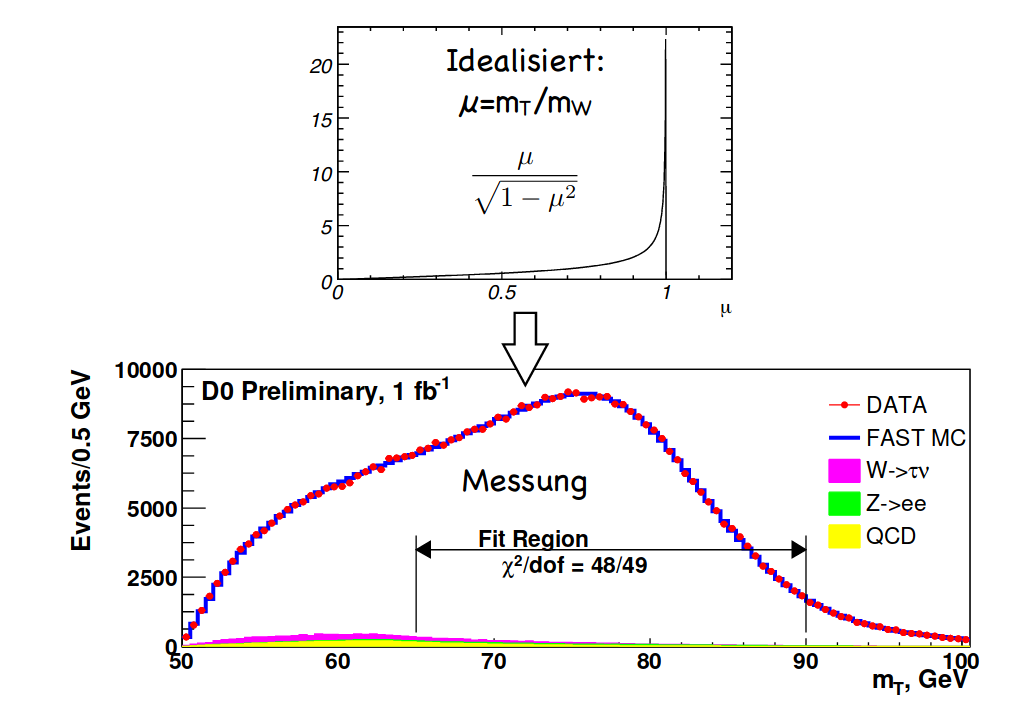
\includegraphics[width=\textwidth]{images/jacobi-peak.png}
        \caption{Darstellung der Jacobi-Kante in idealisierter Form und im Experiment \cite{vorlesung}.}
        % \label{}
      \end{figure}
    \end{column}
    \begin{column}{0.4\textwidth}
      \begin{itemize}
        \item Man erhält für die Jacobi-Determinante dieser Variablentransformation
        \begin{equation*}
          \frac{\symup{d} \cos{(\theta)}}{\symup{d} \mu} = \frac{\symup{d}}{\symup{d}\mu} \sqrt{1-\mu^2} = - \frac{\mu}{\sqrt{1-\mu^2}}
        \end{equation*}
        \item Der differenzielle Wirkungsquerschnitt als Funktion von $m_T$ besitzt damit einen scharfen Knick bei $m_T = m_W$ , den man als "Jacobi-Kante" bezeichnet
      \end{itemize}
    \end{column}
  \end{columns}
\end{frame}

\begin{frame}
  \begin{itemize}
    \item Eine Jacobi-Kante tritt analog auch im differenziellen Wirkungsquerschnitt $\frac{\symup{d} \sigma}{\symup{d} p_T}$ bei einem Transversalimpuls von $p_T = \frac{m_w}{2}$ auf
    \item Im Experiment ist Jacobi-Kante verschmiert
    \begin{itemize}
      \item[\rightarrow] W-Boson wird i.A. nicht in Ruhe erzeugt
      \item[\rightarrow] W-Boson besitzt endliche Zerfallsbreite
      \item[\rightarrow] Detektorauflösung
      \item[\rightarrow] Unsicherheiten in der Rekonstruktion
    \end{itemize}
  \end{itemize}
\end{frame}

\section{Tevatron}

\subsection{Allgemeines}

\begin{frame}{Allgemeines}
    \begin{itemize}
      \item Betrieb durch das Fermilab (Batavia, Illinois)
      \item Proton-Antiproton-Beschleuniger
      \item der sträkste Beschleuniger nach dem LHC am CERN
      \item Schwerpunktsenergie: $\SI{1,96}{\TeV}$
      \item Umfang: $\SI{6}{\km}$
      \item Run I:
      \begin{itemize}
        \item $31.08.1992$ - $20.02.1996$
        \item integrierte Luminosität: $\SI{180}{\pico \barn^{-1}}$
      \end{itemize}
      \item Run II:
      \begin{itemize}
        \item $01.03.2001$ - $29.09.2011$
        \item integrierte Luminosität: $\SI{10}{\femto \barn^{-1}}$ pro Detektor
      \end{itemize}
      \item stillgelegt seit $29.09.2011$
    \end{itemize}
\end{frame}

\subsection{Beschleuniger-Kette}

\begin{frame}
  \begin{figure}
    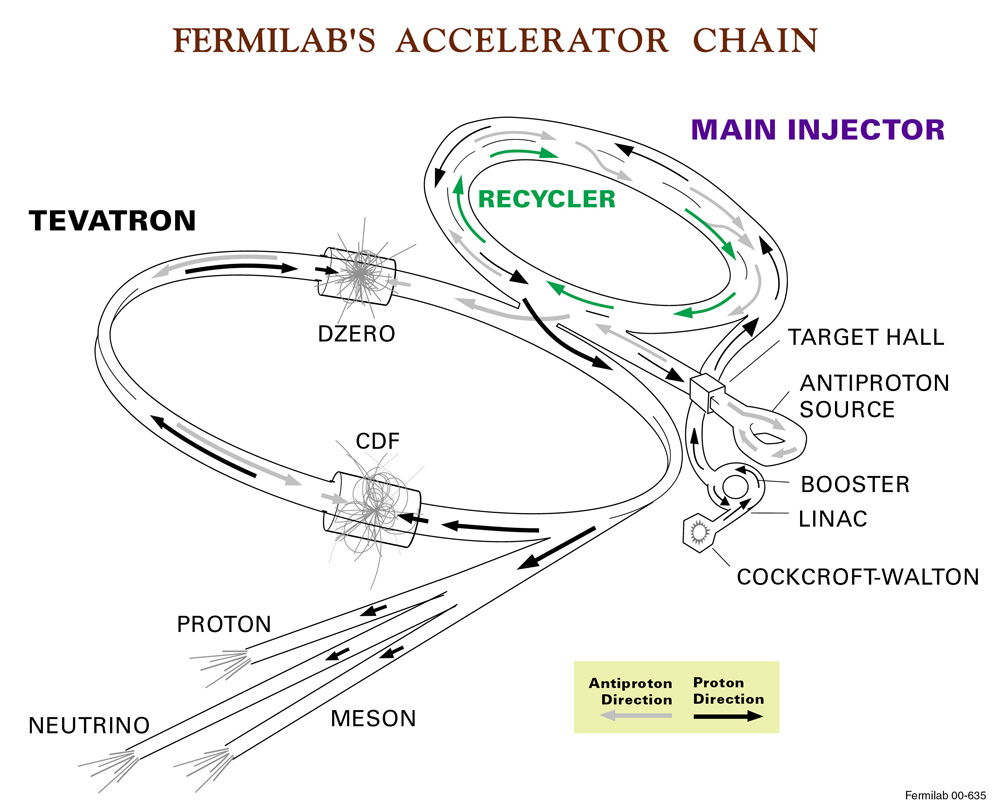
\includegraphics[width=0.55\textwidth]{images/accelerator_chain.jpg}
    \caption{Beschleuniger-Kette am Fermilab \cite{accelerator_chain}.}
    % \label{}
  \end{figure}
\end{frame}

\subsection{Detektoren}

\subsubsection{CDF}

\begin{frame}{CDF}
    \begin{figure}
      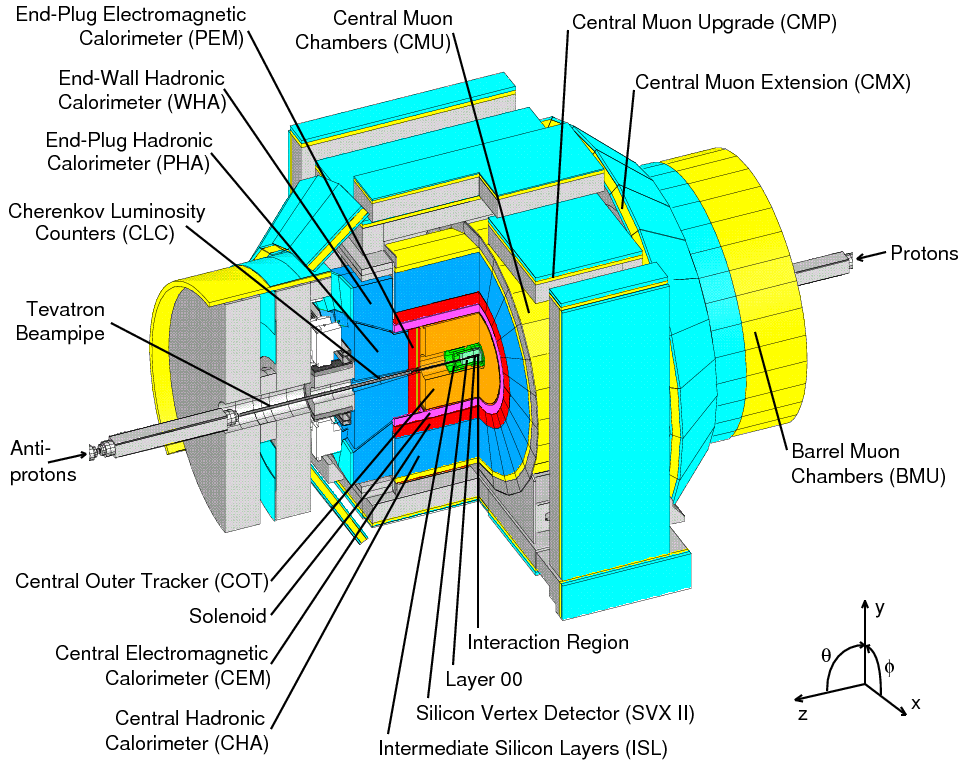
\includegraphics[width=0.55\textwidth]{images/CDF.png}
      \caption{Schematischer Aufbau des CDF-Detektors \cite{CDF_aufbau}}
      % \label{}
    \end{figure}
\end{frame}


\subsubsection{D0}

\begin{frame}{D0}
  \begin{figure}
    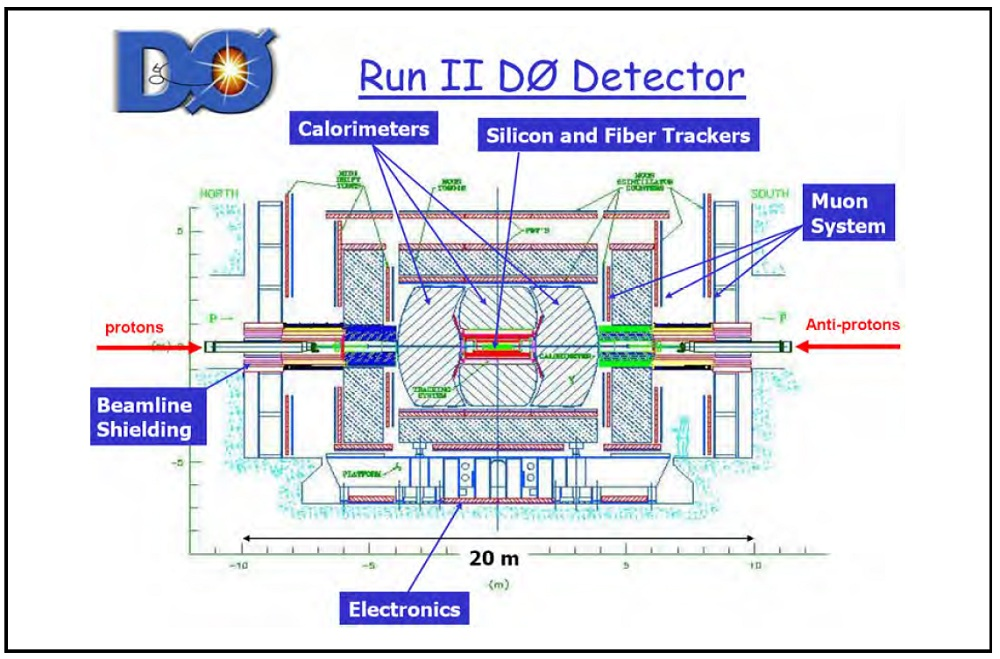
\includegraphics[width=0.65\textwidth]{images/d0.jpg}
    \caption{Schematischer Aufbau des D0-Detektors \cite{D0}}
    % \label{}
  \end{figure}
\end{frame}

\section{Messstrategie und Unsicherheiten am Beispiel von CDF Run II Daten}

\subsection{Event Generation}

\begin{frame}{Event Generation}
  \begin{itemize}
    \item wichitge Größen:
    \begin{itemize}
      \item[\rightarrow] Teilimpulse der Valenzquarks
      \item[\rightarrow] Transversalimpuls des W-Bosons $p_T$
    \end{itemize}
    \item Die Teilimpulse werden mithilfe von globalen Fits auf Hoch-Energie-Daten constrained und als Parton-Verteilungsfunktionen (PDF) dargestellt
    \item Die PDFs werden von unabhängigen Kollaborationen parametrisiert
    \item Die Unsicherheit bei Nutzung einer Parametrisierung der CTEQ (The Coordinated Theoretical-Experimental Project on QCD) liegt bei $\delta m_W(PDF) = \SI{15}{\MeV}$
  \end{itemize}


  % There are two important components of W boson production for measuring m W : the fractional
  % momenta of u and d quarks inside the proton, and the W p T . The u and d momenta determine
  % p W
  % z , which affects the m T distribution. The u and d fractional momenta are constrained from
  % global fits to high-energy data and embodied in parton distribution functions (PDFs) indepen-
  % dently parametrized by the CTEQ 6 and MRST 7 collaborations. Using a CTEQ prescription
  % for obtaining PDF uncertainties, the CDF collaboration has estimated δm W (P DF ) = 15 MeV.


\end{frame}

\begin{frame}
  \begin{itemize}
    \item Die Verteilung von $p_T$ wird durch einen Event Generator (resbos 8) simuliert
    \item Die benötigten Parameter werden überwiegend durch die $p_T$-Messung des Z-Bosons aus Run I constrained
    \item Die Unsicherheit der resbos-Parameter beträgt damit $\delta m_W (p^W_T) = \SI{13}{\MeV}$
  \end{itemize}

  % The W boson p T distribution is predicted by an event generator (resbos 8) that combines a
  % QCD next-to-leading-log calculation with three non-perturbative parameters fit from high energy
  % data. The dominant constraint on these parameters comes from the Z boson p T measurement in
  % Run 1. The generator and detector simulation predict the observed Run 2 Z boson p T spectrum
  % well (Fig. 1). The uncertainty on the resbos parameters results in δm W (p W
  % T ) = 13 MeV.

\end{frame}

\begin{frame}
  \begin{itemize}
    \item Im W-Zerfall hat das Abstrahlen eines Photons durch ein Lepton im Endzustand den größten Effekt auf die W-Massenmessung
    % \item Den größten Effekt auf die Rekonstruktion der W-Masse hat das Abstrahlen eines Photons durch ein Endzustandstlepton
    \item Durch das Abstrahlen verringert sich der Impuls des Leptons wodurch eine geringere W-Masse rekonstruiert wird
    \item Dies wird mithilfe von Simulationen korrigiert
    \item Nicht simuliert werden Photonemissionen im Anfangszustand, Interferenz und Terme höherer Ordnung
    \item[\rightarrow] Daraus folgt eine Unsicherheit von $\num{20}$ ($\num{15}$) $\si{\MeV}$ für den $\mu$- ($e$-) Kanal

    % In the W decay, the most important effect for the W mass measurement is the radiation
    % of a γ from a final-state l ± . This radiation results in a reduced l ± momentum, potentially
    % affecting the inferred mass of the W boson. CDF bases its simulation of final-state radiation
    % on a QED next-to-leading order event generator (wgrad). Effects from initial-state radiation,
    % interference, and higher-order terms are not simulated, resulting in a 20 (15) MeV uncertainty
    % for the m W measurement in the μ (e) channel.
  \end{itemize}
\end{frame}

\subsection{Track Momentum Calibration}

\begin{frame}{Track Momentum Calibration}
  \begin{itemize}
    \item Der Impuls eines geladenen Teilchens wird durch seine Ablenkung im Tracker bestimmt
    \item Da $p \sim \frac{1}{r}$, wird der Impuls als eine Funktion des inversen Impulses des $J/\psi$ skaliert
    \item Um die Auflösung zu verbessern wird die Position des Strahls bei Myon-Spuren von W- und Z-Zerfällen beim Track-Fit mitberücksichtigt
  \end{itemize}
  A charged particle’s momentum is measured through its observed curvature in the tracker.
  Since the momentum is inversely proportional to curvature, the momentum scale is measured
  as a function of the mean inverse momentum of J/ψ muons and fit to a line. The line has zero
  slope, verifying the applicability of the extracted scale to W boson decays.
  To improve momentum resolution, muon tracks from W and Z decays use the beam position
  as a point in the track fit. This constraint cannot be applied to J/ψ decays since they can be
  separated from the beam line. Instead, Υ decays are used to verify that the beam constraint
  produces no bias on the momentum calibration. A systematic uncertainty of 15 MeV accounts
  for the observed difference in scale. Including the uncertainty due to tracker alignment, CDF
  estimates an uncertainty of δm W (p T scale) = 25 MeV.
\end{frame}

\subsection{Calorimeter Energy Calibration}

\begin{frame}{Calorimeter Energy Calibration}
  \begin{itemize}
    \item Das elektromagnetische Kalorimeter wird mithilfe der Elektronen-Tracks aus den W-Zerfällen kalibriert
    \item
  \end{itemize}


  Given the momentum calibration, electron tracks from W decays are used to calibrate the
  electromagnetic calorimeter. The calorimeter energy is scaled such that the ratio of energy
  to track momentum (E/p) is equal to 1. To correct for an energy-dependent scale, the E/p
  distribution is fit as a function of electron E T and a correction applied.
  The significant amount of material in the silicon detector inside the tracker affects the posi-
  tion of the E/p peak. An uncertainty on the amount of material translates into an uncertainty
  on the measured E scale. The fraction of events in the region 1.19 < E/p < 1.85 is a mea-
  sure of the material. The extent to which this region is not well modelled results in a 55 MeV
  uncertainty on the W mass. This uncertainty dominates the total δm W (E scale) of 70 MeV.
\end{frame}

\subsection{Hadronic Recoil Measurement and Simulation}

\begin{frame}{Hadronic Recoil Measurement and Simulation}
  The hadronic recoil energy is measured by vectorially summing all the energy in the calorimeter,
  excluding that contributed by the l. The detector response to the hadronic energy is defined as R = u meas /u true , where u true is the recoil energy of the W boson. The response is measured
using Z → ll, since the l is measured more precisely than the hadronic energy.
The hadronic energy resolution is modelled as having a component from the underlying event
(independent of recoil) and a component from the recoiling hadrons. The model parameters are
tuned using the resolution of Z → ll along the axis bisecting the leptons. This axis is the least
susceptible to fluctuations in l energy. The recoil response and resolution uncertainty on the W
mass is 50 MeV, of which 37 MeV is due to the model of the underlying energy resolution.
\end{frame}

\subsection{Backgrounds}

\begin{frame}{Backgrounds}
  \begin{itemize}
    \item Häufiger Untergrund bei $W \rightarrow e \nu$ und $W \rightarrow \mu \nu$ Zerfällen
    \begin{itemize}
      \item $Z \rightarrow \ell \ell$, wobei ein $\ell$ nicht rekonstruiert wird
      \item $W \rightarrow \tau \nu \rightarrow \ell \nu \nu \nu$
      \item Dijet-Produktion, wobei ein hadronischer Jet als $\ell$ rekonstruiert wird
    \end{itemize}
    \item Im $\mu$-Sample kommt noch Untergrund aus der kosmischen Strahlung hinzu
  \end{itemize}
  % \begin{columns}
    % \begin{column}{0.4\textwidth}
%
    % \end{column}
    % \begin{column}{0.4\textwidth}
%
    % \end{column}
  % \end{columns}


  % The backgrounds common to the W → eν and W → μν samples are: Z → ll, where one l is not
  % reconstructed; W → τ ν → l3ν; and dijet production, with one hadronic jet misreconstructed as
  % an l. In addition, the μ sample includes background from cosmic rays and decays in flight. The
  % W and Z backgrounds are estimated using Monte Carlo. The dijet background estimation uses
  % events with significant energy surrounding the l to enhance hadronic background and obtain a
  % / T distribution is then fit using the W and jet distribu-
  % / T distribution. The data E
  % background E
  % tions as input. The cosmic ray background is determined using track hit timing information and
  % / T ) distribution to a combination
  % the decay-in-flight background estimated by fitting the ∆φ(l, E
  % of W and decay-in-flight distributions. These estimates result in δm W (background) = 20 MeV.
\end{frame}
\begin{frame}
  \begin{itemize}
    \item Die W- und Z-Untergründe werden mithilfe von Monte-Carlo-Simulationen abgeschätzt
    \item Die Abschätzung des Dijet-Untergrundes nutzt Events mit signifikanter Energie um $\ell$ herum, um den hadronischen Untergrund zu erhöhen und eine $\cancel{\it{E}}_{T}$-Verteilung für den Untergrund zu gewinnen
    \item[\rightarrow] Die $\cancel{\it{E}}_{T}$-Verteilung wird mit den W- und Dijet-Verteilungen als Input gefittet
    \item Der Untergrund aufgrund von kosmischer Strahlung wird mithilfe der Track-Hit Zeiten abgeschätzt
    \item Insgesamt ergibt sich eine Unsicherheit von $\delta m_W (\text{background}) = \SI{20}{\MeV}$
  \end{itemize}
\end{frame}

\subsection{Mass Fit and Systematics}

\begin{frame}{Mass Fit and Systematics}
  Given the energy calibrations, recoil model, and background estimation, the m T distribution is
 fit for the e and μ channels. The predicted line shape agrees with that of the data (Fig. 1).
 The central value is blinded while CDF cross-checks the analysis with independent data sets
 and simulation. Combining the two channels (Table 1) results in δm W = 76 MeV.
\end{frame}

\begin{frame}{Zusammenfassung}
  \begin{figure}
    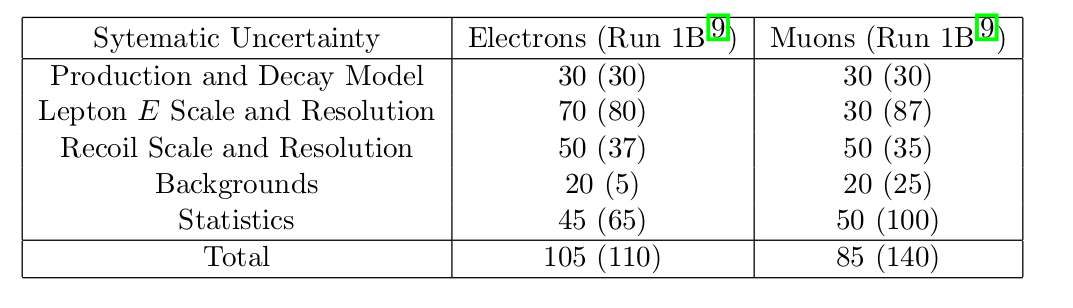
\includegraphics[width=\textwidth]{images/unsicherheiten.png}
    \caption{Unsicherheiten der W-Massenmessung in $\frac{\si{\MeV}}{c^2}$ bei der Nutzung von $\SI{0,2}{\femto \barn^{-1}}$ von CDF Run 2 Daten. In Klammern sind die Unsicherheiten aus CDF Run 1B.}
    % \label{}
  \end{figure}
\end{frame}




% \begin{frame}{Transversale Größen}
 % \begin{columns}
   % \begin{column}{0.4\textwidth}
     % Text,    der    in    der    ersten    Spalte    steht
   % \end{column}
   % \begin{column}{0.4\textwidth}
     % Text,    der    in    der    zweiten    Spalte    steht
   % \end{column}
 % \end{columns}
% \end{frame}

% \section{Test}
%
% \begin{frame}
  % \begin{beamercolorbox}[center, wd=\textwidth]{titlegraphic}
    % 
\includegraphics[width=0.3\textwidth]{images/particle_zoo.jpg}
  % \end{beamercolorbox}%
% \end{frame}

\section{Literatur}
\begin{frame}[allowframebreaks]{Literatur}
  \printbibliography
\end{frame}

\end{document}
